\section{\textbf{Dependencies in Dyadic Data}}

In working with relational data, scholars typically begin by structuring it as a set of dyadic observations stacked on top of one another. This makes sense if each observation is independent of the others. For example, a conflict sent from the United States to Japan, is assumed to be independent of any action that Japan may send to the United States. Additionally, every action sent by Japan to others in the system is considered independent even though each of those interactions involves a common sender, i.e, Japan. While the assumption that most begin with is that each dyadic interaction is taking place in isolation of the others, we know this assumption to be false in theory and in practice. Relational data comes with an explicit structure that generally leads to particular types of dependencies. The importance of accounting for the underlying structure of our data has been a lesson well understood, at least, when it comes to time-series cross-sectional data (TSCS) within political science \citep{beck:katz:1995,beck:etal:1998}. As a result, it is now standard practice to take explicit steps to account for the complex data structures that emerge in TSCS applications and the unobserved heterogeneity that they cause. To uncover the underlying structure of relational data, it is helpful to shift towards restructuring dyadic data in the form of a matrix---often referred to as an adjacency matrix---as shown in Figure~\ref{fig:adjMatDeps}. Rows designate the senders of an event and columns the receivers. The cross-sections in this matrix represent the actions that were sent by an actor in the row to those designated in the columns. Thus $y_{ij}$ designates an action $y$, such as a conflictual event or trade flow, that is sent from actor $i$ to actor $j$. 

Using the structure of an adjacency matrix, Figure~\ref{fig:adjMatDeps} visualizes the types of first- and second-order dependencies that can complicate the analysis of relational data in traditional GLMs. The adjacency matrix on the top left highlights a particular row to illustrate that these values may be more similar to each other than other values because each has a common sender. Interactions involving a common sender also manifest heterogeneity in how active actors are across the network when compared to each other. In most relational datasets (e.g., trade flows, conflict, participation in international organizations, even networks derived from Twitter or Facebook), we often find that there are some actors that are much more active than others \citep{barabasi:reka:1999}. Unless one is able to develop a model that can account for the variety of explanations that may play a role in determining why a particular actor is more active than others, parameter estimates from standard statistical models will be biased.

\begin{figure}
	\begin{tabular}{cc}
		\textsc{Sender heterogeneity} & \textsc{Receiver Heterogeneity} \\
		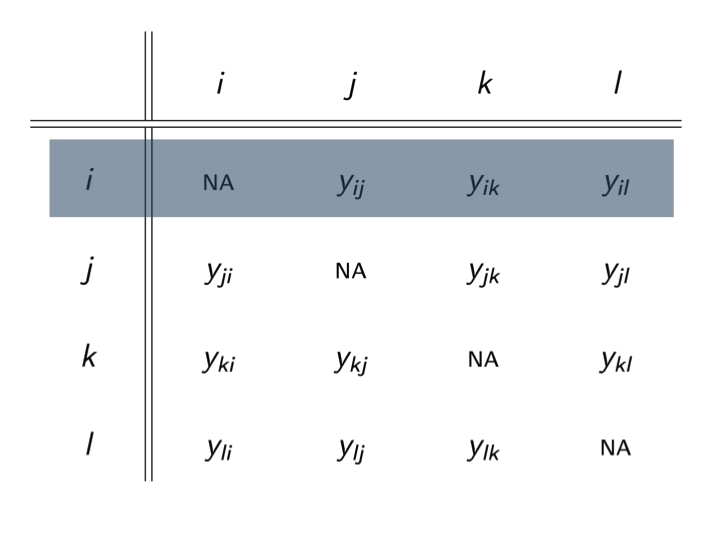
\includegraphics[width=.4\textwidth]{adjRowDep.png} & 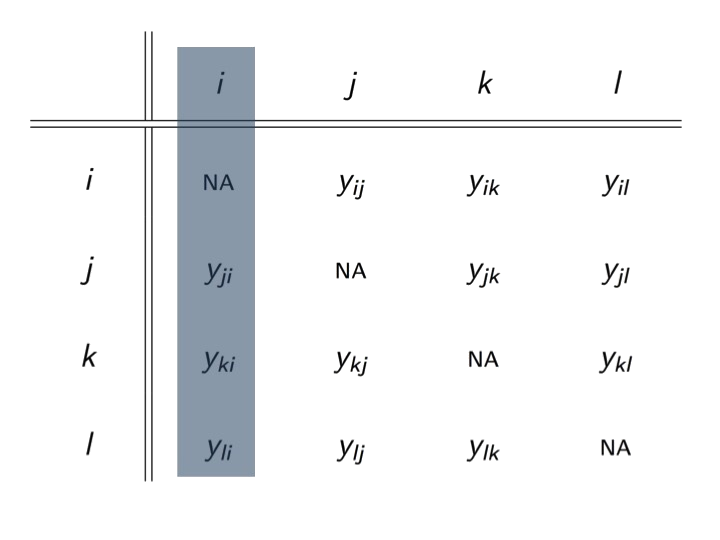
\includegraphics[width=.4\textwidth]{adjColDep.png} \\
		\textsc{Sender-Receiver Covariance} & \textsc{Reciprocity} \\
		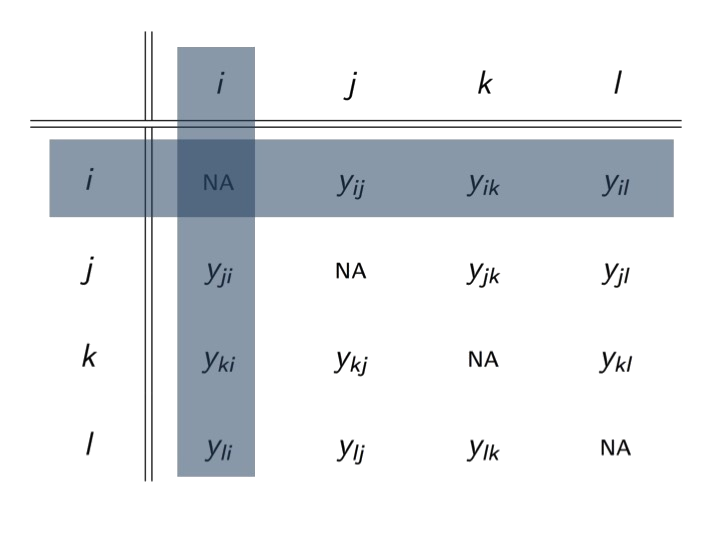
\includegraphics[width=.4\textwidth]{adjRowColCovar.png} & 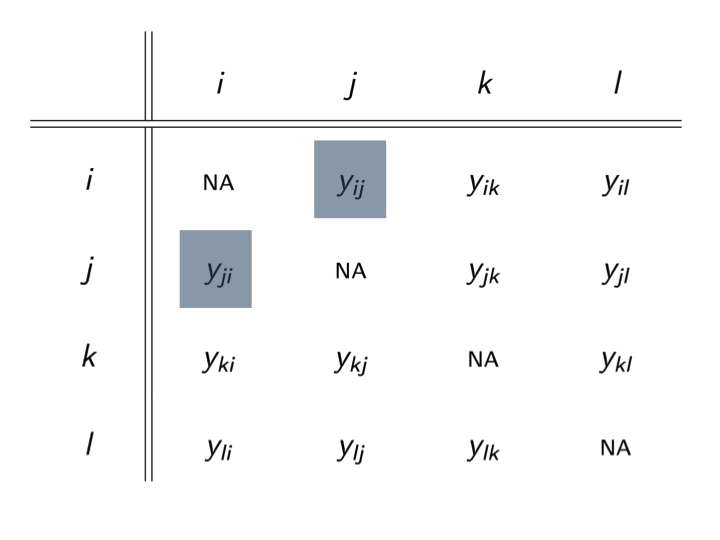
\includegraphics[width=.4\textwidth]{adjRecip.png} \\
	\end{tabular}
	\caption{Nodal and dyadic dependencies in relational data.}
	\label{fig:adjMatDeps}
\end{figure}

For similar reasons one also needs to take into account the shared dependence between observations that share a common receiver. The bottom-left panel in Figure~\ref{fig:adjMatDeps} illustrates that sender and receiver type dependencies can also blend together. Specifically, actors who are more likely to send ties in a network tend to also be more likely to receive them. As a result, the rows and columns in an adjacency matrix are often correlated. For example, consider that trade flows both from and to many wealthy, developed countries. The bottom-right panel highlights a second-order dependence, specifically, reciprocity. This is a dependency occurring within dyads involving the same actors whereby values of $y_{ij}$ and $y_{ji}$ are correlated. The concept of reciprocity has deep roots in the study of relations between states \citep{richardson:1960,keohane:1989}. 

For most relational data, however, dependencies do not simply manifest at the nodal or dyadic level. More often we find significant evidence of higher-order structures that result from dependencies between multiple groups of actors. These dependencies arise because there may be a or some set of latent attributes between actors that affects their probability of interacting with one another \citep{zinnes:1967,wasserman:faust:1994}. In Figure~\ref{fig:thirdDeps} we provide a visualization of a simulated relational dataset wherein the nodes designate actors and edges between the nodes indicate that an interaction between the two took place. To highlight third-order dependence patterns, nodes with similar latent attributes are colored similarly.

\begin{figure}[ht]
	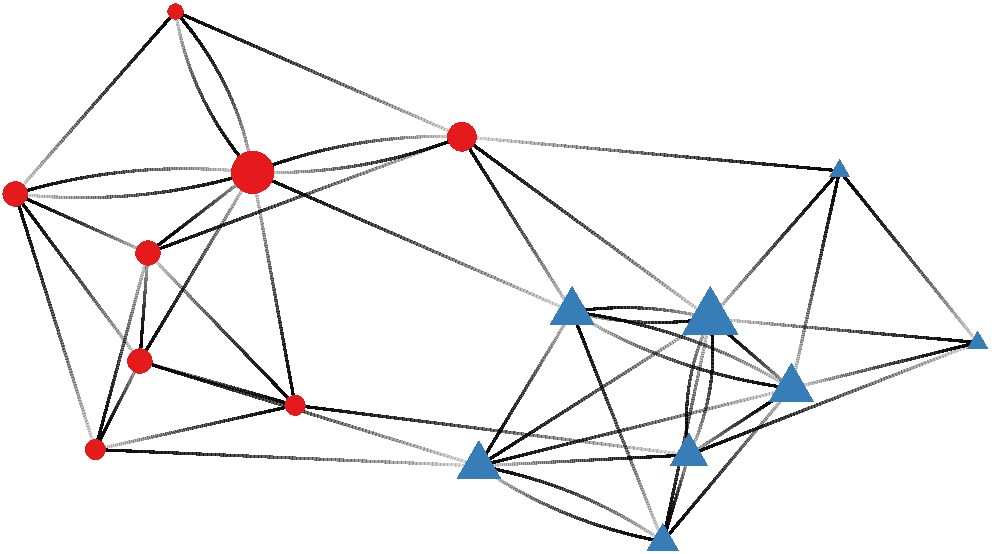
\includegraphics[width=.6\textwidth]{stochEquiv_v2.pdf}
	\caption{Visualization of network with meso-scopic features.}
	\label{fig:thirdDeps}
\end{figure}

The visualization illustrates that the actors belonging to the same group have a higher likelihood of having an interaction with each other, whereas interactions across groups are rarer. A prominent example of a network with this type of structure was found by \citet{adamic:glance:2005}, who visualized the ways in which right and left leaning political blogs linked to one another preceding the 2004 United States Presidential Election. \citeauthor{adamic:glance:2005} find that the degree of interaction between right and left leaning blogs was minimal, and that most blogs linked to others that were politically similar. This showcases the types of higher-order dependencies that can emerge in relational data. First, the fact that interactions were determined by a shared attribute, in this case political ideology, is an example of \textit{homophily}. Homophily explains the emergence of patterns such as transitivity (``a friend of a friend is a friend'') and balance (``an enemy of a friend is an enemy''), which also have a long history in international relations. The other major type of meso-scopic feature that emerges in relational data is community structure \citep{mucha:etal:2010}, which is often formalized through the concept of stochastic equivalence \citep{anderson:etal:1992}. This concept simply refers to the idea that groups of nodes that act similarly in the network are stochastically equivalent. In the example we have laid out above each of the left leaning blogs would be considered stochastically equivalent to one another. 

The presence of these dependencies in relational data points to the fact that there is a complex structure underlying the dyadic events that we observe, and that accounting for this structure is necessary if we are to adequately represent the data generating process. Of course, if one can specify each of the nodal, dyadic, and triadic set of attributes that influence interactions then one can be assured that the conditional independence assumption underlying standard approaches will be satisfied. However, it is rarely the case that we can do this even for TSCS data, thus we often make modeling decisions to account for that structure. Failing to account for the underlying structure in either TSCS or dyadic data leads to a number of well-known challenges: a) biased estimates of the effect of independent variables, b) uncalibrated confidence intervals, and c) poor predictive performance. Further by ignoring these potential interdependencies, we often ignore substantively interesting features of the problem. The study of international relations is founded on the relations among actors. Why ignore the interdependencies that led to the study of IR in the first place?

\section{\textbf{Additive and Multiplicative Effect Models for Networks}}

To account for the dependencies that are prevalent in dyadic data, we turn to the AME model. The AME approach can be used to conduct inference on cross-sectional and longitudinal networks with binary, ordinal, or continuous linkages. It is flexible and easy to use for analyzing the kind of relational data often found in social science. It accounts for nodal and dyadic dependence patterns, as well as higher-order dependencies such as homophily and stochastic equivalence.\footnote{\citet{minhas:etal:2016:arxiv} detail how this framework contrasts with alternative network-based approaches.}

The AME model combines the social relations regression model (SRRM) to account for nodal and dyadic dependencies and the latent factor model (LFM) for third-order dependencies.  For details on the SRRM see \citet{li:loken:2002,dorff:minhas:2017}. An earlier version of the LFM  used in AME is presented as the general bilinear mixed effects (GBME) model in \citet{hoff:ward:2004}. The GBME model is more limited in the types of dependence patterns that it can capture due to the formulation of the matrix decomposition procedure underlying the LFM. The AME model is specified as follows:

\begin{align}
	\begin{aligned}
		y_{ij} \;=\; f(\theta_{ij}) &\text{, where } \\
		\theta_{ij} \;=\;& \bm\beta_{d}^{\top} \mathbf{X}_{ij} + \bm\beta_{s}^{\top} \mathbf{X}_{i} + \bm\beta_{r}^{\top} \mathbf{X}_{j} \text{\qquad(Exogenous parameters)} \\
		& + a_{i} + b_{j} + \epsilon_{ij} \text{\qquad\qquad\qquad\quad(SRRM parameters)} \\
		& + \mathbf{u}_{i}^{\top} \mathbf{D} \mathbf{v}_{j}  \text{\qquad\qquad\qquad\qquad\qquad\;(LFM parameters)} \\ 
	\label{eqn:ame}
	\end{aligned}
\end{align}

where $y_{ij,t}$ captures the interaction between actor $i$ (the sender) and $j$ (the receiver). We use a Bayesian probit framework, in which we model a latent variable, $\theta_{ij}$, using first a set of exogenous dyadic ($\bm\beta_{d}^{\top} \mathbf{X}_{ij}$), sender ($\bm\beta_{s}^{\top} \mathbf{X}_{i}$), and receiver covariates ($\bm\beta_{r}^{\top} \mathbf{X}_{j}$). Next, to account for the dependencies that emerge in dyadic data and that may complicate inference on the parameter associated with exogenous covariates, we add parameters from the SRRM and LFM. $a_{i}$ and $b_{j}$ in Equation~\ref{eqn:ame} represent sender and receiver random effects incorporated from the SRRM framework:

\begin{align}
	\begin{aligned}
		\{ (a_{1}, b_{1}), \ldots, (a_{n}, b_{n}) \} &\simiid N(0,\Sigma_{ab}) \\ 
		\{ (\epsilon_{ij}, \epsilon_{ji}) : \; i \neq j\} &\simiid N(0,\Sigma_{\epsilon}), \text{ where } \\
		\Sigma_{ab} = \begin{pmatrix} \sigma_{a}^{2} & \sigma_{ab} \\ \sigma_{ab} & \sigma_{b}^2   \end{pmatrix} \;\;\;\;\; &\Sigma_{\epsilon} = \sigma_{\epsilon}^{2} \begin{pmatrix} 1 & \rho \\ \rho & 1  \end{pmatrix}
	\label{eqn:srm}
	\end{aligned}
\end{align}

The sender and receiver random effects are modeled jointly from a multivariate normal distribution to account for correlation in how active an actor is in sending and receiving ties. Heterogeneity in the the sender and receiver effects is captured by $\sigma_{a}^{2}$ and $\sigma_{b}^{2}$, respectively, and $\sigma_{ab}$ describes the linear relationship between these two effects (i.e., whether actors who send [receive] a lot of ties also receive [send] a lot of ties). Beyond these first-order dependencies, second-order dependencies are described by $\sigma_{\epsilon}^{2}$ and a within dyad correlation, or reciprocity, parameter $\rho$.

The LFM contribution to the AME comes in the multiplicative term: $\mathbf{u}_{i}^{\top} \mathbf{D} \mathbf{v}_{j}=\sum_{k \in K} d_{k} u_{ik} v_{jk}$. $K$ denotes the dimensions of the latent space. This model posits a latent vector of characteristics $\mathbf{u_{i}}$ and $\mathbf{v_{j}}$ for each sender $i$ and receiver $j$. The similarity or dissimilarity of these vectors will then influence the likelihood of activity, and provides a representation of third-order interdependencies \citep{minhas:etal:2016:arxiv}. The LFM parameters are estimated by a process similar to computing the singular value decomposition (SVD) of the observed network. When taking the SVD we factorize our observed network into the product of three matrices: $\mathbf{U}, \mathbf{D}, \text{ and }, \mathbf{V}$. This provides us with a low-dimensional representation of our original network.\footnote{The dimensions of $\mathbf{U}$ and $\mathbf{V}$ are $n \times K$ and $\mathbf{D}$ is a $K \times K$ diagonal matrix.} Values in $\mathbf{U}$ provide a representation of how stochastically equivalent actors are as senders in a network or, for example, how similar actors are in terms of who they initiate conflict with. $\hat{\mathbf{u}}_{i} \approx \hat{\mathbf{u}}_{j}$ would indicate that actor $i$ and $j$ initiate battles with similar third actors. $\mathbf{V}$ provide a similar representation but from the perspective of how similar actors are as receivers. The values in $\mathbf{D}$, a diagonal matrix, represent levels of homophily in the network.\footnote{Unlike traditional SVD, in the latent factor model, the singular values are not restricted to be positive, thus allowing us to account for both the presence and absence of homophily.}

Note that this model easily generalizes to the case, common in international relations, where interactions are unidrected (for example the presence of conflict or a bilateral investment treaty). In this case, $\rho$ is constrained to be 1, sender and receiver effects are identical for each observation, as are $\mathbf{u_{i}}$ and $\mathbf{v_{j}}$. In the application section, we show the applicability of the AME approach to both directed and undirected dyadic data.

By integrating the SRRM and LFM into a Bayesian probit framework, we can account for the underlying structure in dyadic data that if left unestimated would complicate any inferences we might wish to draw for the exogenous parameters. Parameter estimation in the AME takes place within the context of a Gibbs sampler in which we iteratively sample from the posterior distribution of the full conditionals for each parameter. Specifically, given initial values of $\{\bm\beta, \mathbf{a}, \mathbf{b}, \mathbf{U}, \mathbf{V}, \Sigma_{ab}, \rho, \text{ and } \sigma_{\epsilon}^{2}\}$, the algorithm proceeds as follows until convergence:

 \begin{itemize}
 	\item sample $\bm\theta \; | \;  \bm\beta, \mathbf{X}, \bm\theta, \mathbf{a}, \mathbf{b}, \mathbf{U}, \mathbf{V}, \Sigma_{ab}, \rho, \text{ and } \sigma_{\epsilon}^{2}$ (Normal)
 	\item sample $\bm\beta \; | \;  \mathbf{X}, \bm\theta, \mathbf{a}, \mathbf{b}, \mathbf{U}, \mathbf{V}, \Sigma_{ab}, \rho, \text{ and } \sigma_{\epsilon}^{2}$ (Normal)
 	\item sample $\mathbf{a}, \mathbf{b} \; | \; \bm\beta, \mathbf{X}, \bm\theta, \mathbf{U}, \mathbf{V}, \Sigma_{ab}, \rho, \text{ and } \sigma_{\epsilon}^{2}$ (Normal)
	\item sample $\Sigma_{ab} \; | \; \bm\beta, \mathbf{X}, \bm\theta, \mathbf{a}, \mathbf{b}, \mathbf{U}, \mathbf{V}, \rho, \text{ and } \sigma_{\epsilon}^{2}$ (Inverse-Wishart)
 	\item update $\rho$ using a Metropolis-Hastings step with proposal $p^{*} | p  \sim$ truncated normal$_{[-1,1]}(\rho, \sigma_{\epsilon}^{2})$
 	\item sample $\sigma_{\epsilon}^{2} \; | \; \bm\beta, \mathbf{X}, \bm\theta, \mathbf{a}, \mathbf{b}, \mathbf{U}, \mathbf{V}, \Sigma_{ab}, \text{ and } \rho$ (Inverse-Gamma)
 	\item For each $k \in K$:
 	\begin{itemize}
 		\item Sample $\mathbf{U}_{[,k]} \; | \; \bm\beta, \mathbf{X}, \bm\theta, \mathbf{a}, \mathbf{b}, \mathbf{U}_{[,-k]}, \mathbf{V}, \Sigma_{ab}, \rho, \text{ and } \sigma_{\epsilon}^{2}$ (Normal)
 		\item Sample $\mathbf{V}_{[,k]} \; | \; \bm\beta, \mathbf{X}, \bm\theta, \mathbf{a}, \mathbf{b}, \mathbf{U}, \mathbf{V}_{[,-k]}, \Sigma_{ab}, \rho, \text{ and } \sigma_{\epsilon}^{2}$ (Normal)
 		\item Sample $\mathbf{D}_{[k,k]}  \; | \; \bm\beta, \mathbf{X}, \bm\theta,\mathbf{a}, \mathbf{b}, \mathbf{U}, \mathbf{V}, \Sigma_{ab}, \rho, \text{ and } \sigma_{\epsilon}^{2}$ (Normal)\footnote{Subsequent to estimation, $\mathbf{D}$ matrix is absorbed into the calculation for $\mathbf{V}$ as we iterate through $K$. }
 	\end{itemize}
 \end{itemize}
